% Appendix E: Build and Deployment Evidence
\chapter{Build and Deployment Evidence}
\label{app:build}

This appendix documents the build configuration, dependency inventory, and
deployment artefacts produced for the OrderVista project.

%--------------------------------------------------------------
\section{Build Environment}

\begin{table}[H]
\centering
\caption{Build and development environment.}
\label{tab:build-env}
\begin{tabular}{@{}ll@{}}
\toprule
\textbf{Component} & \textbf{Version / Detail}\\
\midrule
Flutter SDK       & 3.35.2 (stable channel) \\
Dart SDK          & $\geq$\,3.0.0, $<$\,4.0.0 \\
Android Gradle Plugin & 8.9.1 \\
Kotlin            & 2.1.0 \\
Compile SDK       & 36 (Android 16) \\
Target SDK        & 35 (Android 15) \\
Min SDK           & 26 (Android 8.0 Oreo) \\
Java compatibility & 1.8 (desugared with \texttt{desugar\_jdk\_libs 2.1.4}) \\
Development OS    & Windows 10/11 \\
IDE               & Visual Studio Code with Flutter/Dart extensions \\
Version control   & Git + GitHub (branch-per-feature) \\
\bottomrule
\end{tabular}
\end{table}

%--------------------------------------------------------------
\section{Android Release Build}

The signed release APK was produced using the following command:

\begin{verbatim}
flutter build apk --release
\end{verbatim}

\begin{table}[H]
\centering
\caption{Release APK details.}
\label{tab:release-apk}
\begin{tabular}{@{}ll@{}}
\toprule
\textbf{Property} & \textbf{Value}\\
\midrule
Application ID    & \texttt{com.ordervista.dispatch} \\
Version name      & 1.0.0 \\
Version code      & 1 \\
APK size          & 75.7\,MB \\
Signing           & Release keystore (SHA-256 signed) \\
ProGuard          & Enabled (default rules) \\
\bottomrule
\end{tabular}
\end{table}

\begin{figure}[H]
\centering
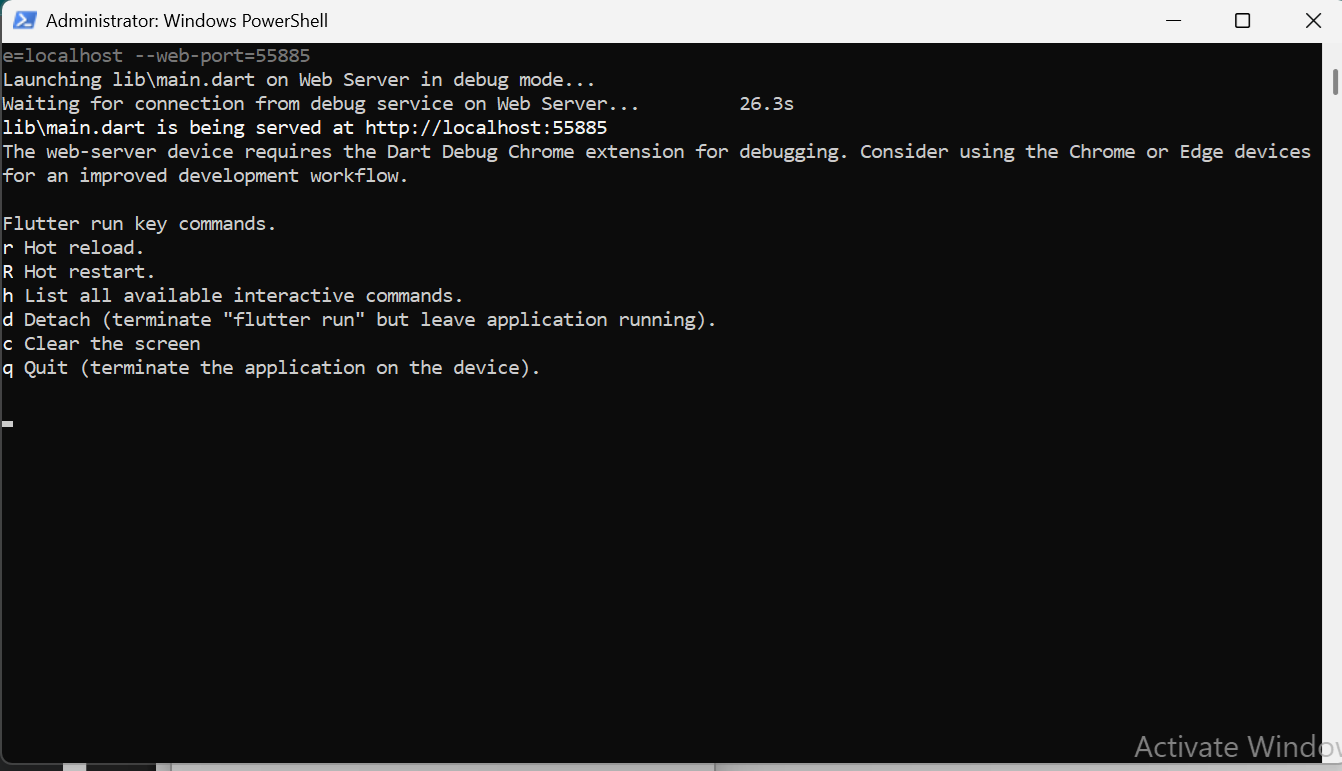
\includegraphics[width=0.7\textwidth]{ss-build-output}
\caption{Terminal output of a successful \texttt{flutter build apk --release}.}
\label{fig:build-output}
\end{figure}

%--------------------------------------------------------------
\section{Backend Deployment}

\begin{table}[H]
\centering
\caption{Supabase project configuration.}
\label{tab:supabase-config}
\begin{tabular}{@{}ll@{}}
\toprule
\textbf{Setting} & \textbf{Value}\\
\midrule
Hosting          & Supabase Cloud (free tier) \\
Region           & Southeast Asia \\
PostgreSQL       & 15.x with PostGIS extension \\
Authentication   & Supabase Auth (email/password) \\
Storage          & Supabase Storage (PoD photos) \\
Realtime         & Enabled for \texttt{chat\_messages} and \texttt{tasks} \\
Migrations       & 3 SQL migration files (see Appendix~\ref{app:schema}) \\
\bottomrule
\end{tabular}
\end{table}

%--------------------------------------------------------------
\section{External Service Configuration}

\begin{table}[H]
\centering
\caption{External API integrations.}
\label{tab:ext-apis}
\begin{tabular}{@{}lll@{}}
\toprule
\textbf{Service} & \textbf{Purpose} & \textbf{Plan}\\
\midrule
Mapbox Geocoding API   & Address $\to$ coordinates & Free tier \\
Mapbox Static Images   & Route map previews       & Free tier \\
OpenRouter API         & LLM gateway              & Pay-per-token \\
DeepSeek R1            & AI model (via OpenRouter) & Free tier \\
\bottomrule
\end{tabular}
\end{table}

%--------------------------------------------------------------
\section{Dependency Inventory}

Table~\ref{tab:deps} lists the principal Dart/Flutter packages used.

\begin{small}
\begin{longtable}{@{}llp{7cm}@{}}
\caption{Key project dependencies.}
\label{tab:deps}\\
\toprule
\textbf{Package} & \textbf{Version} & \textbf{Purpose}\\
\midrule
\endfirsthead
\toprule
\textbf{Package} & \textbf{Version} & \textbf{Purpose}\\
\midrule
\endhead
\bottomrule
\endlastfoot

\texttt{supabase\_flutter}    & 2.3.4  & Supabase client (auth, DB, storage, realtime) \\
\texttt{drift}                & 2.18.0 & SQLite ORM for offline cache \\
\texttt{sqlite3\_flutter\_libs} & 0.5.22 & Native SQLite bindings \\
\texttt{go\_router}           & 12.1.3 & Declarative routing with role guards \\
\texttt{provider}             & 6.1.5  & State management (ChangeNotifier) \\
\texttt{geolocator}           & 11.0.0 & GPS location services \\
\texttt{mobile\_scanner}      & 4.0.1  & Barcode and QR code scanning \\
\texttt{image\_picker}        & 1.1.2  & Camera photo capture \\
\texttt{csv}                  & 6.0.0  & CSV parsing for bulk import \\
\texttt{file\_picker}         & 10.3.8 & File selection dialog \\
\texttt{cached\_network\_image} & 3.4.1 & Image caching with placeholders \\
\texttt{google\_fonts}        & 6.1.0  & Typography \\
\texttt{flutter\_animate}     & 4.5.0  & Declarative animations \\
\texttt{intl}                 & 0.20.2 & Date/number formatting \\
\texttt{timeago}              & 3.7.1  & Relative time display \\
\texttt{url\_launcher}        & 6.3.1  & External link/map navigation \\
\texttt{shared\_preferences}  & 2.5.3  & Key-value persistent storage \\
\texttt{json\_path}           & 0.7.2  & JSON querying for AI responses \\
\end{longtable}
\end{small}

%--------------------------------------------------------------
\section{Repository Structure}

\begin{verbatim}
ordervista/
  lib/
    main.dart               # Entry point
    app/                    # App shell, theme, router
    bootstrap/              # Initialisation, DI
    config/                 # AppConfig, environment
    data/                   # Drift database, DAOs
    models/                 # Domain models
    repositories/           # Repository pattern layer
    services/               # Supabase, Mapbox, AI services
    viewmodels/             # MVVM view-models
    screens/                # Admin portal screens
    pages/                  # Driver app pages
    components/             # Shared UI components
  supabase/
    migrations/             # 3 SQL migration files
  android/                  # Android build config
  test/                     # Unit and widget tests
  pubspec.yaml              # Dependencies
\end{verbatim}

%--------------------------------------------------------------
\section{Web Deployment}
\label{sec:web-deploy}

The admin portal is deployed as a Flutter Web release on Vercel.
The production URL is:

\begin{center}
\url{https://ordervista.vercel.app}
\end{center}

The web build was compiled with environment variables baked in at build time
using \texttt{flutter build web --release --dart-define-from-file=.env}.
A \texttt{vercel.json} rewrite rule ensures that Flutter's client-side
routing functions correctly on page refresh and deep links.

%--------------------------------------------------------------
\section{Google Play Store Submission}
\label{sec:play-store}

A signed Android App Bundle (\texttt{app-release.aab}, 55.9\,MB) was uploaded
to Google Play Console under the closed testing track.  At the time of
writing, 12~testers have been recruited and the mandatory 14-day closed
testing period required by Google for new developer accounts is in progress.
Production access will be requested upon completion of this review period.

%--------------------------------------------------------------
\section{Evaluation Access Credentials}
\label{sec:eval-creds}

Table~\ref{tab:eval-creds} provides test credentials for evaluators to
access the live deployment.  These accounts are provisioned on the project's
Supabase instance and are intended solely for examination purposes.

\begin{table}[H]
\centering
\caption{Evaluation credentials for the live system.}
\label{tab:eval-creds}
\begin{tabular}{@{}llll@{}}
\toprule
\textbf{Role} & \textbf{Email} & \textbf{Password} & \textbf{Access Point}\\
\midrule
Admin / Dispatcher & \texttt{abed-al-rahman@cityu.com} & \texttt{profgerhardcs4514} & \url{https://ordervista.vercel.app} \\
Driver             & \texttt{worker2@gmail.com}          & \texttt{worker2}          & Android APK \\
Driver             & \texttt{worker3@gmail.com}          & \texttt{worker3}          & Android APK \\
Driver             & \texttt{worker4@gmail.com}          & \texttt{worker4}          & Android APK \\
Driver             & \texttt{worker5@gmail.com}          & \texttt{worker5}          & Android APK \\
\bottomrule
\end{tabular}
\end{table}

\noindent\textbf{Note:} The admin portal is accessible via web browser.  The
driver application requires the signed Android APK installed on a physical
device (GPS and camera features are not available in browser).
